% TODO: 
% check again if the text are smooth enough from paragraph or from sub points to another sub points (Check the ChatGPT under "Hausarbeit überarbeiten unerquicklich")

\documentclass[runningheads]{res/llncs}

\usepackage[T1]{fontenc}
\usepackage[utf8]{inputenc}
\usepackage[ngerman]{babel}
\usepackage{graphicx}
\usepackage{subcaption}
\usepackage{float}
\usepackage{tabularx}
\usepackage{booktabs}
\usepackage{url}
% Makes citations, URLs, table of contents entries and cross-references clickable in the PDF.
% Use hidelinks for a clean academic style without colored boxes.
\usepackage[ngerman]{babel}
\usepackage{hyperref}
\usepackage[acronym,nonumberlist,section=section]{glossaries}
% Sortierung durch LaTeX; kein separater makeglossaries-Aufruf erforderlich.
\makenoidxglossaries
% Zentrale Definitionen des Abkürzungsverzeichnisses.
% Im Haupttext: \gls{etcs} (erste Verwendung ausgeschrieben),
% \acrshort{etcs} (nur Abkürzung), \acrlong{etcs} (nur Langform).
% Neue Einträge werden automatisch im Verzeichnis aufgeführt.

\newacronym[description={Zweite Mobilfunkgeneration (\textit{Second Generation})},sort={2g}]{2g}{2G}{Zweite Mobilfunkgeneration (\textit{Second Generation})}
\newacronym[description={\textit{Triple Data Encryption Standard}; dreifache Anwendung des DES-Verfahrens},sort={3des}]{3des}{3DES}{Triple Data Encryption Standard}
\newacronym[description={\textit{3rd Generation Partnership Project}; Standardisierungsgremium für Mobilfunksysteme},sort={3gpp}]{3gpp}{3GPP}{3rd Generation Partnership Project}
\newacronym[description={Fünfte Mobilfunkgeneration (\textit{Fifth Generation})},sort={5g}]{5g}{5G}{Fünfte Mobilfunkgeneration (\textit{Fifth Generation})}
\newacronym[description={Sechste Mobilfunkgeneration (\textit{Sixth Generation})},sort={6g}]{6g}{6G}{Sechste Mobilfunkgeneration (\textit{Sixth Generation})}
\newacronym[description={Verschlüsselungsalgorithmen der GSM-Funkschnittstelle},sort={a51}]{a51}{A5/1}{Verschlüsselungsalgorithmen der GSM-Funkschnittstelle}
\newacronym[description={Verschlüsselungsalgorithmen der GSM-Funkschnittstelle},sort={a53}]{a53}{A5/3}{Verschlüsselungsalgorithmen der GSM-Funkschnittstelle}
\newacronym[description={\textit{Automatic Train Control}; automatische Zugsteuerung},sort={atc}]{atc}{ATC}{Automatic Train Control}
\newacronym[description={\textit{Advanced Train Administration and Communications System}; funkbasiertes Zugsteuerungssystem von JR East},sort={atacs}]{atacs}{ATACS}{Advanced Train Administration and Communications System}
\newacronym[description={\textit{Automatic Train Operation}; automatisierter Zugbetrieb},sort={ato}]{ato}{ATO}{Automatic Train Operation}
\newacronym[description={\textit{Balise Transmission Module}; fahrzeugseitiges Modul zum Empfang von Eurobalisen-Telegrammen},sort={btm}]{btm}{BTM}{Balise Transmission Module}
\newacronym[description={\textit{Base Transceiver Station}; Basisstation eines Mobilfunknetzes},sort={bts}]{bts}{BTS}{Base Transceiver Station}
\newacronym[description={\textit{Cipher Block Chaining}; Betriebsart einer Blockchiffre},sort={cbc}]{cbc}{CBC}{Cipher Block Chaining}
\newacronym[description={\textit{Communications-Based Train Control}; kommunikationsbasierte Zugsteuerung},sort={cbtc}]{cbtc}{CBTC}{Communications-Based Train Control}
\newacronym[description={\textit{Control-Command and Signalling}; Zugsteuerung, Zugsicherung und Signalgebung},sort={ccs}]{ccs}{CCS}{Control-Command and Signalling}
\newacronym[description={\textit{Cryptography Research and Evaluation Committees}; japanisches Gremium zur Bewertung kryptographischer Verfahren},sort={cryptrec}]{cryptrec}{CRYPTREC}{Cryptography Research and Evaluation Committees}
\newacronym[description={\textit{Digital Automatic Train Control}; digitale Ausprägung der automatischen Zugsteuerung},sort={d-atc}]{d-atc}{D-ATC}{Digital Automatic Train Control}
\newacronym[description={\textit{Data Encryption Standard}; älterer symmetrischer Verschlüsselungsalgorithmus},sort={des}]{des}{DES}{Data Encryption Standard}
\newacronym[description={\textit{Driver Machine Interface}; Anzeige- und Bedienschnittstelle im Führerraum},sort={dmi}]{dmi}{DMI}{Driver Machine Interface}
\newacronym[description={\textit{European Rail Traffic Management System}; europäischer Rahmen für interoperable Zugsteuerung und Signalgebung},sort={ertms}]{ertms}{ERTMS}{European Rail Traffic Management System}
\newacronym[description={\textit{European Train Control System}; europäisches Zugsteuerungs- und Zugsicherungssystem innerhalb von ERTMS},sort={etcs}]{etcs}{ETCS}{European Train Control System}
\newacronym[description={\textit{European Vital Computer}; sicherheitskritischer ETCS-Fahrzeugrechner},sort={evc}]{evc}{EVC}{European Vital Computer}
\newacronym[description={\textit{Future Railway Mobile Communication System}; Nachfolgesystem von GSM-R},sort={frmcs}]{frmcs}{FRMCS}{Future Railway Mobile Communication System}
\newacronym[description={\textit{Grade of Automation 4}; vollautomatischer, unbegleiteter Zugbetrieb},sort={goa4}]{goa4}{GoA4}{Grade of Automation 4}
\newacronym[description={\textit{Global System for Mobile Communications -- Railway}; eisenbahnspezifisches Mobilfunksystem},sort={gsm-r}]{gsm-r}{GSM-R}{Global System for Mobile Communications -- Railway}
\newacronym[description={\textit{Home Location Register}; zentrale Teilnehmerdatenbank eines GSM-Netzes},sort={hlr}]{hlr}{HLR}{Home Location Register}
\newacronym[description={\textit{Hash-based Message Authentication Code} auf Basis von SHA-256},sort={hmac-sha256}]{hmac-sha256}{HMAC-SHA256}{\textit{Hash-based Message Authentication Code} auf Basis von SHA-256}
\newacronym[description={\textit{Intrusion Detection System}; System zur Angriffserkennung},sort={ids}]{ids}{IDS}{Intrusion Detection System}
\newacronym[description={\textit{International Electrotechnical Commission}; internationale elektrotechnische Normungsorganisation},sort={iec}]{iec}{IEC}{International Electrotechnical Commission}
\newacronym[description={\textit{Internet Protocol}; Netzwerkprotokoll für paketvermittelte Kommunikation},sort={ip}]{ip}{IP}{Internet Protocol}
\newacronym[description={\textit{International Organization for Standardization}; internationale Normungsorganisation},sort={iso}]{iso}{ISO}{International Organization for Standardization}
\newacronym[description={Informationstechnik},sort={it}]{it}{IT}{Informationstechnik}
\newacronym[description={\textit{Japanese National Railways}; frühere staatliche japanische Eisenbahngesellschaft},sort={jnr}]{jnr}{JNR}{Japanese National Railways}
\newacronym[description={\textit{Japan Railways}; Gruppe der aus der JNR hervorgegangenen Eisenbahnunternehmen},sort={jr}]{jr}{JR}{Japan Railways}
\newacronym[description={Symmetrischer EuroRadio-Schlüssel zur Bildung eines \textit{Message Authentication Code}},sort={kmac}]{kmac}{KMAC}{Symmetrischer EuroRadio-Schlüssel zur Bildung eines \textit{Message Authentication Code}}
\newacronym[description={\textit{Key Management Centre}; Stelle zur Verwaltung und Verteilung kryptographischer Schlüssel},sort={kmc}]{kmc}{KMC}{Key Management Centre}
\newacronym[description={\textit{Key Management System}; System zur Verwaltung kryptographischer Schlüssel},sort={kms}]{kms}{KMS}{Key Management System}
\newacronym[description={\textit{ETCS Level 2 without Signals}; ETCS Level 2 ohne ortsfeste Lichtsignale},sort={l2os}]{l2os}{L2oS}{ETCS Level 2 without Signals}
\newacronym[description={\textit{Leaky Coaxial Cable}; Schlitz- beziehungsweise Leckkabel zur Funkversorgung entlang der Strecke},sort={lcx}]{lcx}{LCX}{Leaky Coaxial Cable}
\newacronym[description={\textit{Lineside Electronic Unit}; streckenseitige elektronische Einheit zur Ansteuerung von Eurobalisen},sort={leu}]{leu}{LEU}{Lineside Electronic Unit}
\newacronym[description={Leit- und Sicherungstechnik},sort={lst}]{lst}{LST}{Leit- und Sicherungstechnik}
\newacronym[description={\textit{Movement Authority}; ETCS-Fahrterlaubnis},sort={ma}]{ma}{MA}{Movement Authority}
\newacronym[description={\textit{Message Authentication Code}; kryptographischer Prüfwert für Integrität und Authentizität einer Nachricht},sort={mac}]{mac}{MAC}{Message Authentication Code}
\newacronym[description={\textit{Mission-Critical Services}; 3GPP-Dienste für missionskritische Kommunikation},sort={mcx}]{mcx}{MCx}{Mission-Critical Services}
\newacronym[description={\textit{Multiple Independent Levels of Security}; Architekturprinzip zur strikten Isolation von Systempartitionen},sort={mils}]{mils}{MILS}{Multiple Independent Levels of Security}
\newacronym[description={\textit{Moving Target Defense}; dynamische Veränderung von Systemparametern zur Erschwerung von Angriffen},sort={mtd}]{mtd}{MTD}{Moving Target Defense}
\newacronym[description={\textit{On-Board Unit}; fahrzeugseitige Steuerungs- und Kommunikationseinheit},sort={obu}]{obu}{OBU}{On-Board Unit}
\newacronym[description={\textit{Public Key Infrastructure}; Infrastruktur zur Verwaltung digitaler Zertifikate und Schlüssel},sort={pki}]{pki}{PKI}{Public Key Infrastructure}
\newacronym[description={\textit{Reliability, Availability, Maintainability and Safety}; Zuverlässigkeit, Verfügbarkeit, Instandhaltbarkeit und Sicherheit},sort={rams}]{rams}{RAMS}{Reliability, Availability, Maintainability and Safety}
\newacronym[description={\textit{Radio Block Centre}; ETCS-Streckenzentrale zur Erzeugung und Übertragung von Fahrterlaubnissen},sort={rbc}]{rbc}{RBC}{Radio Block Centre}
\newacronym[description={\textit{Railway Mobile Radio}; UIC-Rahmen für den zukünftigen Bahnmobilfunk},sort={rmr}]{rmr}{RMR}{Railway Mobile Radio}
\newacronym[description={\textit{Rail Radio Intrusion Detection System}; Angriffserkennungssystem für CBTC-Funkkommunikation},sort={rrids}]{rrids}{RRIDS}{Rail Radio Intrusion Detection System}
\newacronym[description={\textit{Railway Technical Research Institute}; japanisches Eisenbahnforschungsinstitut},sort={rtri}]{rtri}{RTRI}{Railway Technical Research Institute}
\newacronym[description={\textit{Safety-Critical Application Development Environment}; Entwicklungsumgebung für sicherheitskritische Software},sort={scade}]{scade}{SCADE}{Safety-Critical Application Development Environment}
\newacronym[description={\textit{Secure Hash Algorithm} mit einer Ausgabelänge von 256 Bit},sort={sha-256}]{sha-256}{SHA-256}{\textit{Secure Hash Algorithm} mit einer Ausgabelänge von 256 Bit}
\newacronym[description={\textit{Single Point of Failure}; einzelne Fehlerstelle, deren Ausfall das Gesamtsystem beeinträchtigen kann},sort={spof}]{spof}{SPOF}{Single Point of Failure}
\newacronym[description={\textit{Transmission Control Protocol/Internet Protocol}; grundlegende Protokollfamilie IP-basierter Netze},sort={tcpip}]{tcpip}{TCP/IP}{Transmission Control Protocol/Internet Protocol}
\newacronym[description={\textit{Time Division Multiple Access}; Zeitmultiplexverfahren für den gemeinsamen Zugriff auf einen Funkkanal},sort={tdma}]{tdma}{TDMA}{Time Division Multiple Access}
\newacronym[description={\textit{Train Integrity Monitoring System}; System zur Überwachung der Vollständigkeit eines Zuges},sort={tims}]{tims}{TIMS}{Train Integrity Monitoring System}
\newacronym[description={\textit{Transport Layer Security}; Protokoll zur kryptographischen Absicherung von Netzwerkverbindungen},sort={tls}]{tls}{TLS}{Transport Layer Security}
\newacronym[description={\textit{Telecom On-Board Architecture}; modulare fahrzeugseitige Telekommunikationsarchitektur},sort={toba}]{toba}{TOBA}{Telecom On-Board Architecture}
\newacronym[description={\textit{Train Real-Time Data Protocol}; Kommunikationsprotokoll für Zugnetzwerke},sort={trdp}]{trdp}{TRDP}{Train Real-Time Data Protocol}
\newacronym[description={\textit{Technical Specification for Interoperability relating to Control-Command and Signalling}; europäische Interoperabilitätsspezifikation für Zugsteuerung, Zugsicherung und Signalgebung},sort={tsiccs}]{tsiccs}{TSI CCS}{Technical Specification for Interoperability relating to Control-Command and Signalling}
\newacronym[description={\textit{International Union of Railways} (\textit{Union Internationale des Chemins de fer}); internationaler Eisenbahnverband},sort={uic}]{uic}{UIC}{\textit{International Union of Railways} (\textit{Union Internationale des Chemins de fer})}
\newacronym[description={Drahtlose lokale Netzwerktechnologie},sort={wi-fi}]{wi-fi}{Wi-Fi}{Drahtlose lokale Netzwerktechnologie}
\newacronym[description={Standard für digitale Zertifikate in Public-Key-Infrastrukturen},sort={x509}]{x509}{X.509}{Standard für digitale Zertifikate in Public-Key-Infrastrukturen}
\newacronym[description={\textit{Micro Timed Efficient Stream Loss-tolerant Authentication}; Verfahren zur zeitverzögerten Authentifizierung von Broadcast-Nachrichten},sort={mutesla}]{mutesla}{$\mu$TESLA}{Micro Timed Efficient Stream Loss-tolerant Authentication}
\newacronym[description={\textit{Wireless Local Area Network}; drahtloses lokales Netzwerk},sort={wlan}]{wlan}{WLAN}{Wireless Local Area Network}

\usepackage[backend=biber,style=alphabetic]{biblatex}
\addbibresource{reference.bib}
\addbibresource{Train_ITSec.bib}
\begin{document}
% Langformen sind im Text bereits ausgeschrieben; Abkürzungen bleiben kurz und verlinkt.
\glsunsetall


\title{Kommunikationssicherheit zwischen Zügen und Leitstellen: Eine vergleichende Untersuchung europäischer und japanischer Eisenbahnsysteme}

\titlerunning{Eisenbahn-Kommunikationssicherheit: Europa und Japan}

\author{Agha Muhammad Aslam -- \today}

% \date{\today}

\institute{
Hochschule Fulda \\
Fachbereich Angewandte Informatik \\
\email{agha-muhammad.aslam@informatik.hs-fulda.de}
}

\maketitle

\begin{abstract}
Die zunehmende Digitalisierung der Eisenbahn erhöht die Bedeutung sicherer Zug-Strecken-Kommunikation. Diese Hausarbeit untersucht anhand einer strukturierten Literaturanalyse, wie europäische und japanische Eisenbahnsysteme sicherheitskritische Kommunikation schützen und welche Sicherheitsgrenzen bestehen bleiben. Betrachtet werden insbesondere \gls{ertms}/\gls{etcs}, \gls{gsm-r}, \textit{EuroRadio} und \gls{frmcs} sowie \gls{d-atc}, \gls{atacs} und aktuelle japanische Forschungsansätze. Der Vergleich zeigt unterschiedliche Standardisierungsmodelle, zugleich aber eine gemeinsame Entwicklung hin zur stärkeren Entkopplung sicherheitskritischer Steuerungsfunktionen vom Übertragungsmedium. Kryptographische Verfahren schützen insbesondere Integrität und Authentizität, während die Verfügbarkeit der Kommunikation eine zentrale verbleibende Sicherheitsgrenze darstellt.

\keywords{Eisenbahnsicherheit \and \gls{etcs} \and \gls{ertms} \and \gls{gsm-r} \and \gls{frmcs} \and \gls{atacs} \and \gls{iec} 62280 \and Kommunikationssicherheit}
\end{abstract}

\section{Einleitung und Hintergrund}
\label{sec:Einleitung_und_Hintergrund}

Schienennetze bilden eine gesellschaftlich und wirtschaftlich bedeutsame Verkehrsinfrastruktur, deren zuverlässiger Betrieb Personen- und Güterverkehr sowie die öffentliche Sicherheit betrifft~\parencite[S. 4]{xiangliuCyber2020}. Mit zunehmender Digitalisierung hängt der Bahnbetrieb stärker von Informations-, Leit-, Sicherungs- und Kommunikationssystemen ab~\parencite[S. 3–4]{xiangliuCyber2020}. Fahrzeuge, streckenseitige Einrichtungen und betriebliche Zentralen tauschen dabei unter anderem Fahrterlaubnisse, Positions- und Geschwindigkeitsdaten aus, die unmittelbar zur Steuerung und Überwachung von Zugbewegungen dienen~\parencite[S. 88, 106, 163–166]{trinckaufETCS2024}. Störungen oder Manipulationen dieser Systeme können den Betrieb beeinträchtigen und im schlimmsten Fall die Betriebssicherheit gefährden~\parencite[S. 204, 207]{trinckaufETCS2024}. Entsprechend müssen Kommunikationsverbindungen sowohl gegen Fehler als auch gegen gezielte Angriffe geschützt werden~\parencite[S. 204]{trinckaufETCS2024}. 

Die bundesweite \gls{gsm-r}-Störung vom 23. Juni 2026 verdeutlicht diese Abhängigkeit: Nach dem Austausch eines \textit{Switches} verhinderte ein nicht gemeldeter Softwarefehler die automatische Aktivierung des redundanten Systems. Erst nach Ausschluss eines Cyberangriffs wurde nach rund 90 Minuten manuell auf die Rückfallebene umgeschaltet~\cite{dbinfragoUrsacheZugfunkStoerung2026}. Der Vorfall zeigt, dass neben dem Schutz vor Angriffen auch Redundanz, kontrollierte Wartungsprozesse und wirksames Störungsmanagement für die Sicherheit digitaler Bahnsysteme entscheidend sind.

Europa und Japan verfolgen unterschiedliche architektonische Ansätze. In Europa bildet \gls{ertms} einen interoperablen Rahmen zur Harmonisierung nationaler Signalsysteme und zur Unterstützung des grenzüberschreitenden Eisenbahnbetriebs~\cite{EuropeanCommission_ERTMS_2026}. 

In Japan formulieren nationale Vorgaben überwiegend funktionale und leistungsbezogene Anforderungen, während die Betreiber eigene technische Implementierungsstandards festlegen~\cite{yanaseJapanese2011}. Dadurch können sich Systeme zwischen Betreibern und Strecken unterscheiden; erforderliche Interoperabilität wird über gemeinsame Schnittstellen hergestellt, ohne ein landesweit einheitliches System vorzuschreiben~\cite{MLIT_CBTC_2021}.

Diese Hausarbeit vergleicht ausgewählte europäische und japanische Ansätze der sicherheitskritischen Eisenbahnkommunikation zwischen Zügen und Leitstellen. Die Forschungsfrage lautet: Wie schützen europäische und japanische Eisenbahnsysteme sicherheitskritische Kommunikation zwischen Zügen und Leitstellen, und welche Sicherheitsgrenzen oder Forschungslücken bleiben bestehen? Der Vergleich ist relevant, weil beide Regionen zunehmend digitale, drahtlose und softwaredefinierte Eisenbahnarchitekturen entwickeln, jedoch von unterschiedlichen historischen und technischen Ausgangspunkten ausgehen.

\section{Theoretischer Rahmen}
\label{sec:Theoretischer_Rahmen}

\subsection{Sicherheitskritische Eisenbahnkommunikation}
\label{sec:Sicherheitskritische_Eisenbahnkommunikation}

Sicherheitskritische Eisenbahnkommunikation umfasst die Übertragung von Informationen, die Zugbewegungen oder die betriebliche Sicherheit beeinflussen, etwa \textit{Movement Authorities}, Brems- und Geschwindigkeitsinformationen, Zugpositionsmeldungen oder Notstopp-Nachrichten~\parencite[S. 120–121]{trinckaufETCS2024}. Werden solche Informationen verändert, verzögert, wiederholt oder gefälscht, können Fehlentscheidungen oder restriktive Systemzustände die Folge sein~\parencite[S. 17]{iwamotoTrain2024}. Die Kommunikation ist daher als Bestandteil eines sicherheitskritischen Regelkreises und nicht nur als technischer Datenaustausch zu betrachten.

Vier Sicherheitsziele sind für diese Hausarbeit besonders wichtig. \textbf{Vertraulichkeit} dient dem Schutz vor der unberechtigten Offenlegung von Daten gegenüber Dritten 
% \parencite[S. 207]{trinckaufETCS2024}
. \textbf{Integrität} bedeutet, dass eine Nachricht ohne unbefugte Veränderung ankommen muss. Der Empfänger muss also erkennen können, ob etwa eine \textit{Movement Authority}, ein Geschwindigkeitsprofil oder eine Positionsmeldung manipuliert wurde.
% \parencite[S. 207]{trinckaufETCS2024}
% \parencite[S. 17]{iwamotoTrain2024}
\textbf{Authentizität} stellt sicher, dass Nachrichten zweifelsfrei von einem autorisierten Kommunikationspartner stammen, wie etwa einem \textit{Radio Block Centre} (\gls{rbc}) oder einer \textit{On-Board-Unit} (\gls{obu}).
% \parencite[S. 207]{trinckaufETCS2024}
% \parencite[S. 743]{chothiaAttack2017}
Schließlich muss die \textbf{Verfügbarkeit} der Kommunikation so zuverlässig sein, dass ein sicherer und effizienter Eisenbahnbetrieb gewährleistet bleibt 
\unskip~\parencite[S. 207]{trinckaufETCS2024}
. Dies ist im Bahnbetrieb besonders kritisch, da aufgrund des Prinzips der \textit{Intrinsic Safety} ein Kommunikationsverlust (\textit{Absence of Communication}) unmittelbar dazu führt, dass Züge aus Sicherheitsgründen anhalten oder in einen restriktiven Modus wechseln 
\unskip~\parencite[S. 56]{gaggeroSurvey2024}.
% \parencite[S. 207]{trinckaufETCS2024}.

% PAUSE 09.09.2026 -- Start 09.09.2026 %
Das Verhältnis zwischen \textit{Safety} (funktionaler Sicherheit) und \textit{Security} (\gls{it}-Sicherheit) ist komplex und durch grundlegend verschiedene Zielsetzungen geprägt. Während die \textit{Safety} darauf abzielt, das System so zu gestalten, dass zufällige und systematische Fehler sowie vorhersehbare statistische Einflüsse beherrscht werden, konzentriert sich die \textit{Security} auf den Schutz vor bewussten, manipulativen Eingriffen von außen und innen. 
% \parencite[S. 204]{trinckaufETCS2024}. 
In diesem Sinne kann die \textit{Security} als „Dienstleister“ für die \textit{Safety} betrachtet werden, um die \gls{rams}-Ziele (Zuverlässigkeit -- \textit{Reliability}, Verfügbarkeit -- \textit{Availability}, Instandhaltbarkeit -- \textit{Maintainability} und Sicherheit -- \textit{Safety}) dauerhaft aufrechtzuerhalten~\parencite[S. 204]{trinckaufETCS2024}. 

Ein wesentlicher Unterschied zwischen \textit{Safety} und \textit{Security} liegt in ihrer zeitlichen Dynamik: Während \textit{Safety}-Anforderungen weitgehend langfristig stabil bleiben, müssen \textit{Security}-Maßnahmen aufgrund neuer Technologien und Bedrohungen kontinuierlich angepasst werden~\parencite[S. 204]{trinckaufETCS2024}. Das Zusammenspiel zeigt sich im Prinzip der \textit{Intrinsic Safety}: Bei einem Ausfall sicherheitsrelevanter Kommunikation geht das System in einen restriktiven Zustand, typischerweise bis zum Zughalt~\parencite[S. 56]{gaggeroSurvey2024}. Angriffe auf die Kommunikationsverfügbarkeit, etwa durch \textit{Jamming}, können diese Schutzreaktion gezielt auslösen und dadurch einen \textit{Denial-of-Service}-Zustand mit eingeschränkter betrieblicher Verfügbarkeit verursachen~\parencite[S. 207]{trinckaufETCS2024}~\parencite[S. 56, 59]{gaggeroSurvey2024}.

\subsection{Übersicht gemeinsamer Komponenten funkbasierter Zugsteuerungssysteme}
\label{sec:Übersicht_gemeinsamer_Komponenten_funkbasierter_Zugsteuerungssysteme}

\subsubsection{Systemarchitektur}
\label{sec:Systemarchitektur}
Unabhängig von regionalen Spezifikationen und Herstellern weisen funkbasierte Zugsteuerungssysteme (\textit{Communications-Based Train Control}, \gls{cbtc}) eine gemeinsame grundlegende Systemarchitektur auf~\parencite[S. 9--11]{xiangliuCyber2020}. Die Hauptfunktion besteht darin, eine sichere Zugfolgeabstandshaltung ohne ausschließliche Abhängigkeit von physischen Gleisstromkreisen zu gewährleisten~\parencite[S. 9]{xiangliuCyber2020}. Das Gesamtsystem gliedert sich in folgende zentrale Komponenten:

\begin{figure}[htbp!]
\centering
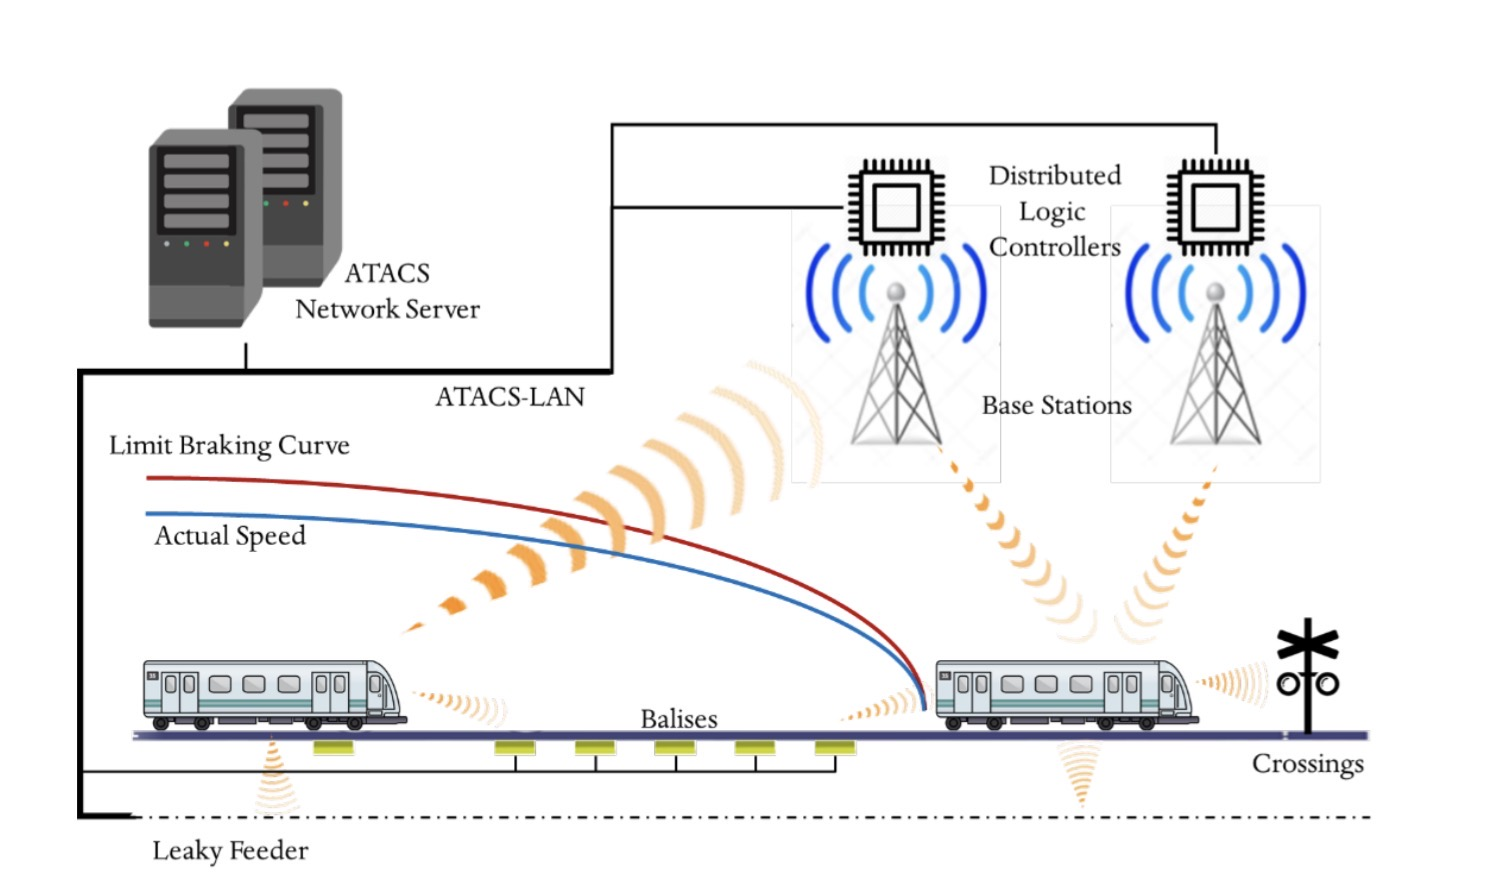
\includegraphics[width=0.65\textwidth]{res/Bahn_Infrastruktur.jpg}
\caption{Überblick über die Schieneninfrastruktur~\cite{xiangliuCyber2020}}
\label{fig:Schieneninfrastruktur}
\end{figure}

\begin{itemize}
    \item \textbf{Fahrzeugseitige Steuerungseinheit (\textit{On-Board Unit} / \gls{evc} / \gls{atc}-Fahrzeuggerät):} Zentraler Sicherheitsrechner, der Geschwindigkeit und Zugposition verarbeitet und daraus die Einhaltung von Fahrterlaubnissen und Bremskurven überwacht~\parencite[S. 10]{xiangliuCyber2020}~\parencite[S. 101--104]{trinckaufETCS2024}. Über das Führerraumdisplay (\textit{Driver Machine Interface}, \gls{dmi}) werden relevante Zustände dem Fahrpersonal angezeigt. Je nach System übernimmt die Einheit überwachende und eingreifende Funktionen bis hin zur automatischen Bremsung~\parencite[S. 14]{xiangliuCyber2020}~\parencite[S. 62--66]{trinckaufETCS2024}.

    \item \textbf{Gleisseitige punktförmige Datenübertrager (Balisen / \textit{Transponder}):} Im Gleis installierte Datenübertrager, die beim Überfahren Telegramme an das Fahrzeug übertragen~\parencite[S. 10--11]{xiangliuCyber2020}~\parencite[S. 75--76]{trinckaufETCS2024}. Sie dienen als Referenzpunkte für die Positionsbestimmung und können je nach System unter anderem Fahrterlaubnisse sowie Geschwindigkeits- und Streckeninformationen übertragen~\parencite[S. 62--63, 75, 79]{trinckaufETCS2024}.

    \item \textbf{Drahtlose Kommunikationsschnittstelle:} Bidirektionale Funkverbindung zwischen Fahrzeug und Strecke zur Übertragung sicherheitsrelevanter Informationen, insbesondere von Positionsberichten und Fahrterlaubnissen~\parencite[S. 9--10]{xiangliuCyber2020}. In Europa wird hierfür insbesondere \gls{gsm-r} eingesetzt; andere Systeme nutzen beispielsweise \gls{tdma}-basierte Funkverfahren oder \textit{Leaky-Coaxial}-Kabel (\gls{lcx})~\parencite[S. 12--14]{xiangliuCyber2020}.

    \item \textbf{Optionale optische Signalisierung:} Ortsfeste Lichtsignale können je nach System und Ausbaustufe ergänzend zur fahrzeugseitigen Signalisierung bestehen bleiben und dem Fahrpersonal eine visuelle Information über den Fahrweg geben~\parencite[S. 10]{xiangliuCyber2020}.
\end{itemize}

% \subsubsection{Schienenmobilfunk der 2. Generation}

\subsubsection{\texorpdfstring{Grundprinzipien generischer Schutzkonzepte: \gls{ids} und \gls{mtd}}{Grundprinzipien generischer Schutzkonzepte: IDS und MTD}}
\label{sec:Grundprinzipien_generischer_Schutzkonzepte_IDS_und_MTD}
Kryptographische Schutzmechanismen sichern die Vertraulichkeit und Authentizität von Nachrichten, bieten jedoch keinen vollständigen Schutz gegen Angriffe auf Netzwerkechzeit und Verfügbarkeit~\parencite[S. 121]{poschingerOpenMTD2020}~\parencite[S. 60]{melaragnoRail2016}. Daher werden komplementäre Schutzkonzepte in die Systemarchitekturen integriert:

\begin{itemize}
    \item \textbf{\textit{Intrusion Detection Systems} (\gls{ids}):} Bahnspezifische Angriffserkennungssysteme (wie \gls{rrids}) analysieren den Funkverkehr auf Protokollebene. Sie vergleichen empfangene Nachrichtenmuster mit mathematischen Zustandsmodellen (z. B. zeitlich gestaffelte Schlüsselketten \textit{via} \gls{mutesla}) und identifizieren Anomalien wie \textit{Replay}-Versuche, Nachrichtenverfälschungen oder \textit{Session-Hijacking}~\parencite[S. 60--63]{melaragnoRail2016}.
    \item \textbf{\textit{Moving Target Defense} (\gls{mtd}):} \gls{mtd}-Verfahren verändern dynamisch Systemparameter der Netzwerkebene während des Betriebs. Durch kontinuierliches Ändern von Portnummern (\textit{Port Hopping}) oder \gls{ip}-Adressen (\textit{Network Address Shuffling}) wird die Relevanz von Netzwerk-\textit{Reconnaissance} durch Dritte reduziert, da gesammelte Zielinformationen nach kurzen Zeitintervallen invalide werden~\parencite[S. 66, 121]{poschingerOpenMTD2020}.
\end{itemize}

\subsection{\texorpdfstring{Europäische Eisenbahnarchitektur: \gls{ertms} und \gls{etcs}}{Europäische Eisenbahnarchitektur: ERTMS und ETCS}}
\label{sec:Europäische_Eisenbahnarchitektur_ERTMS_und_ETCS}

\subsubsection{Struktur und Funktionsweise}
\label{sec:Struktur_und_Funktionsweise}
Das \textit{European Rail Traffic Management System} (\gls{ertms}) definiert das \textit{European Train Control System} (\gls{etcs}) als einheitliches europäisches Zugsicherungssystem~\parencite[S. 49]{trinckaufETCS2024}. Die funktionale Interaktion zwischen Zug und Streckenausrüstung wird über Stufen (\textit{Level}) strukturiert:

\begin{figure}[htbp!]
    \centering
    
    \begin{subfigure}{0.48\textwidth}
    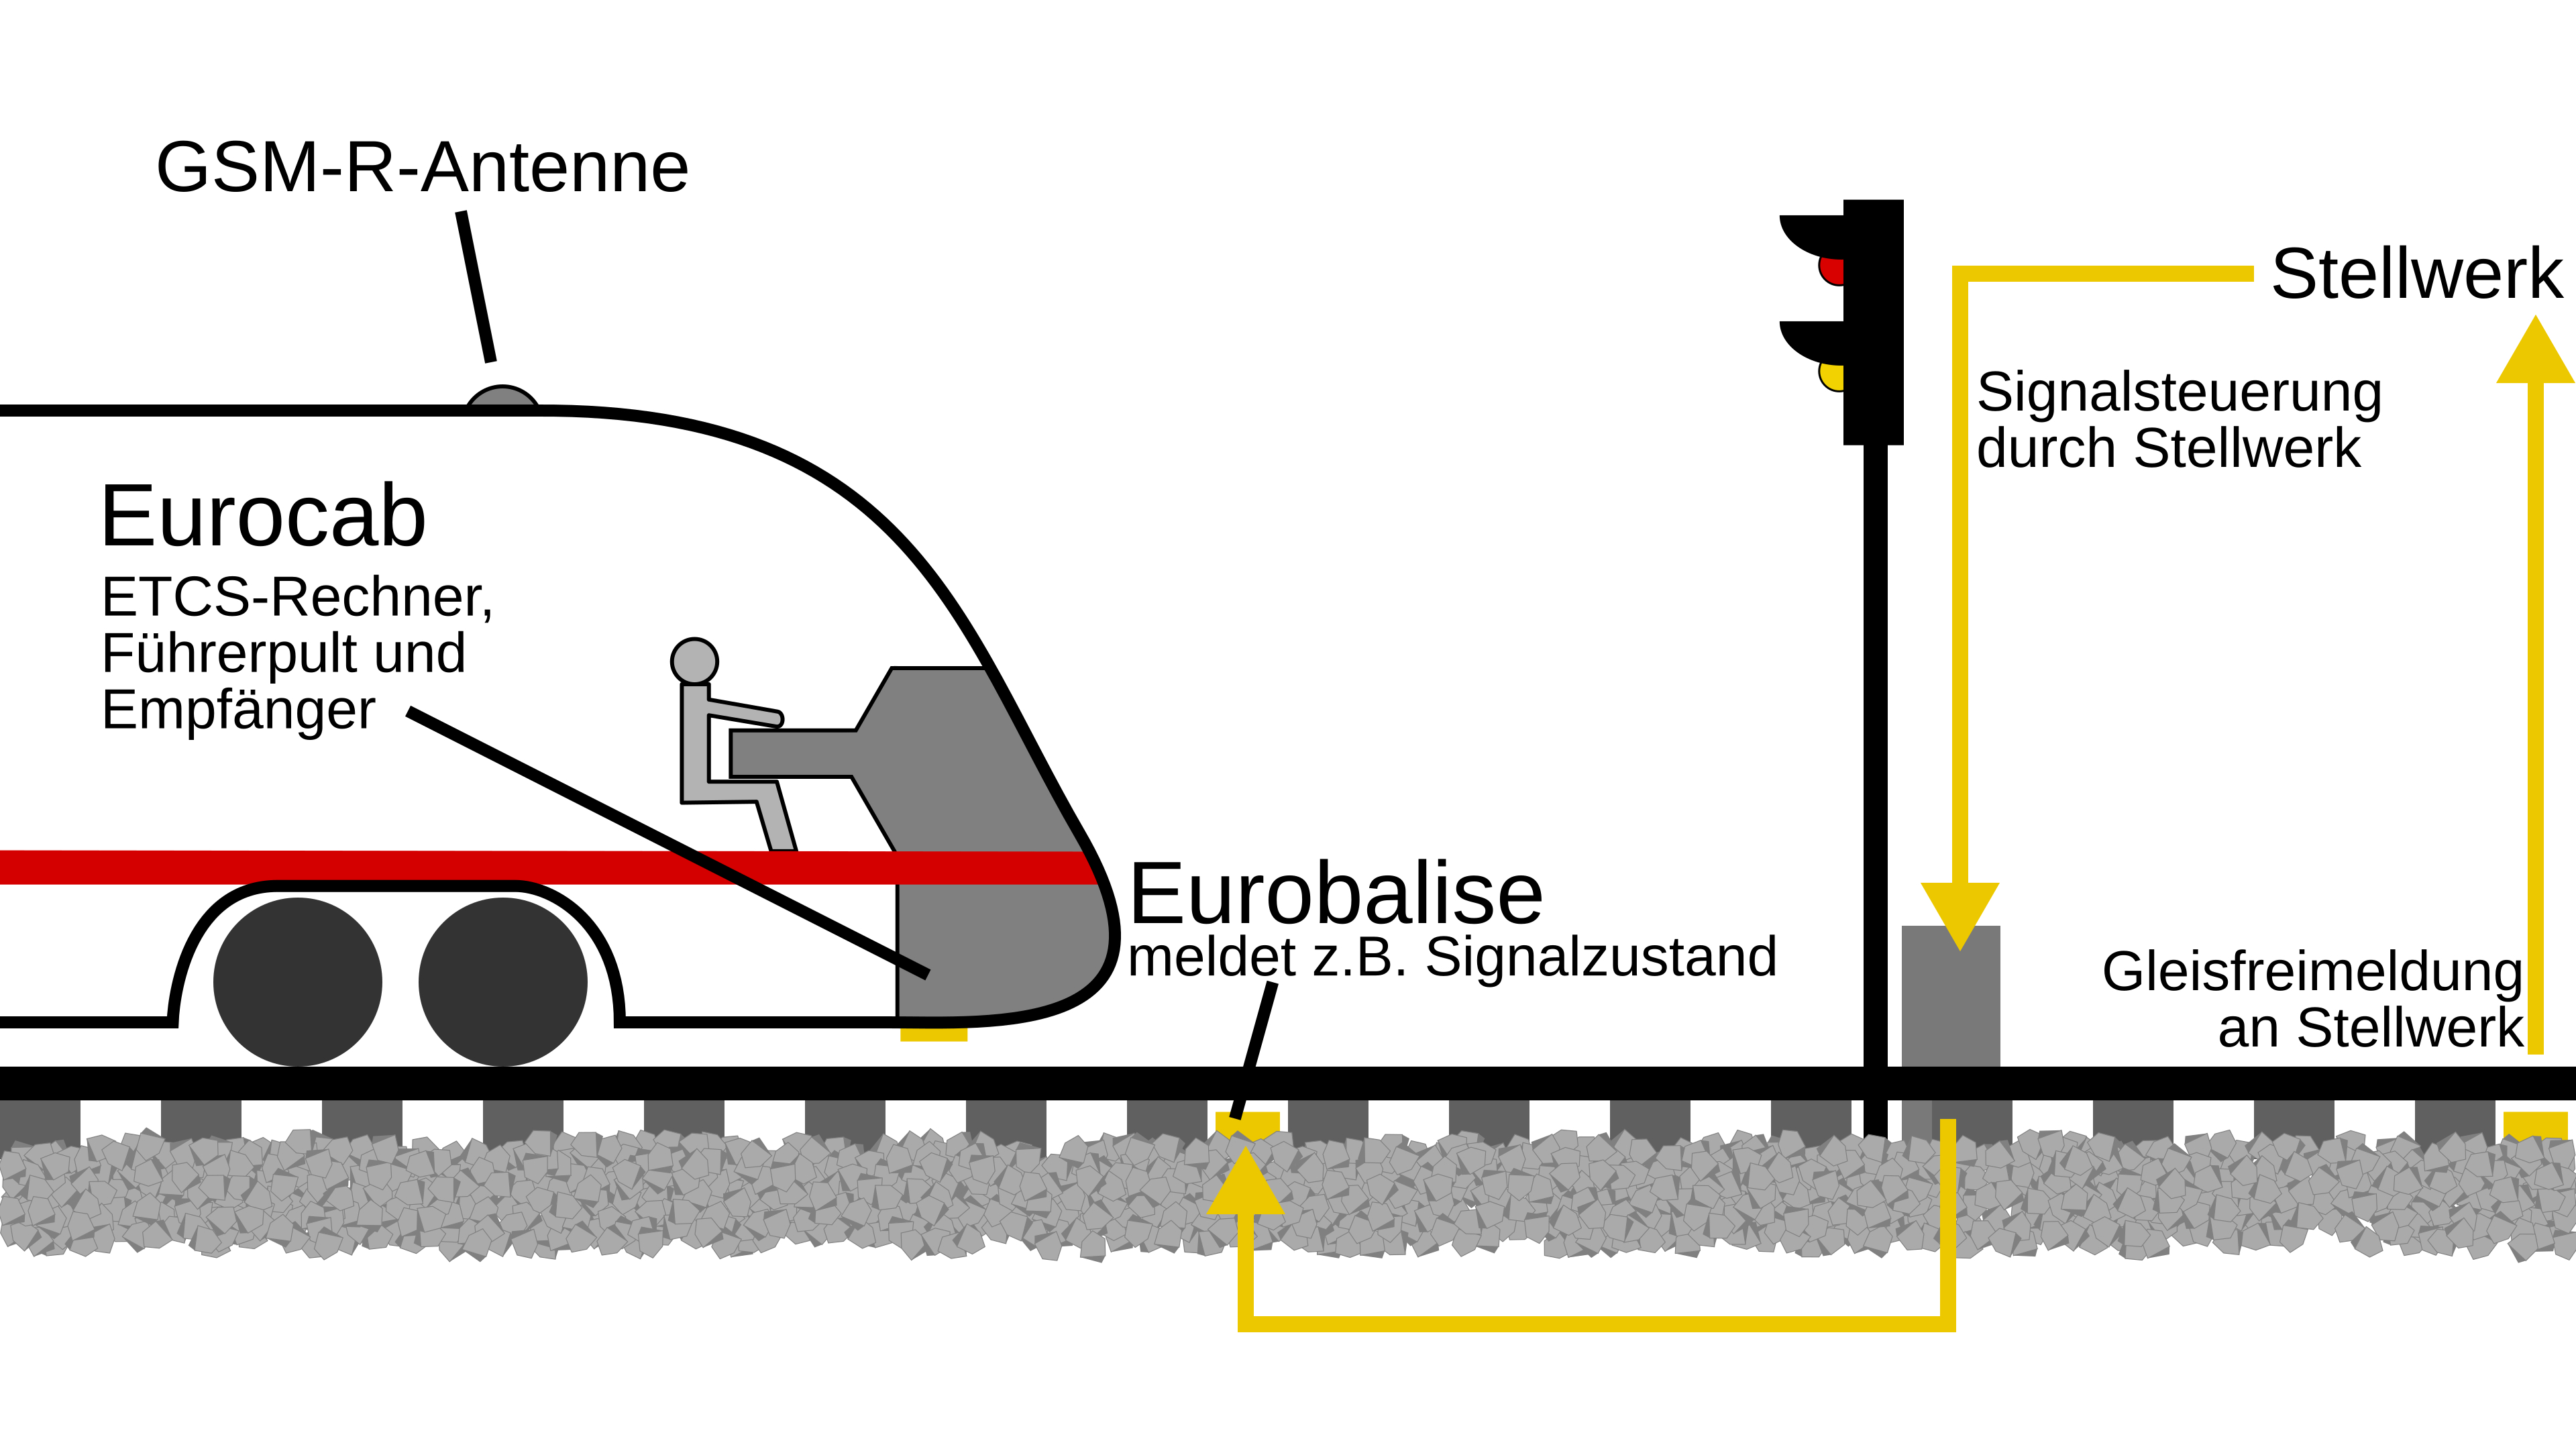
\includegraphics[width=\linewidth]{res/ECTS_Level1.jpg}
    \caption{\gls{etcs} \textit{Level} 1~\cite{sansculotteETCSLevel1}}
    \label{fig:ETCS-level-1}
    \end{subfigure}
    \hfill
    \begin{subfigure}{0.48\textwidth}
    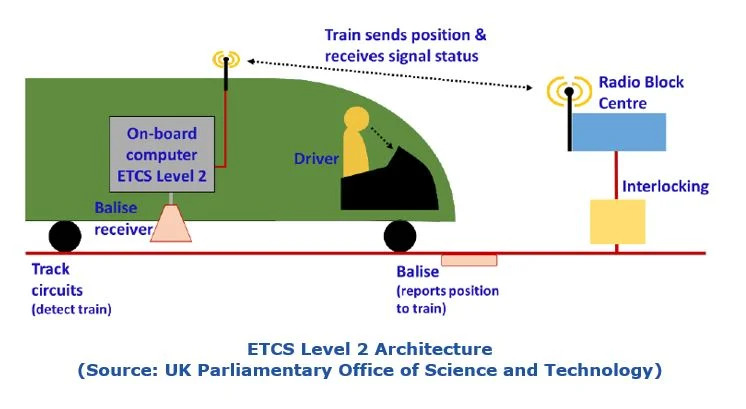
\includegraphics[width=\linewidth]{res/ECTS_Level2.jpg}
    \caption{\gls{etcs} \textit{Level} 2~\cite{arcETCS}}
    \label{fig:ETCS-level-2}
    \end{subfigure} 

\end{figure}

\begin{itemize}

    % \begin{figure}[htbp!]
    % \centering
    % 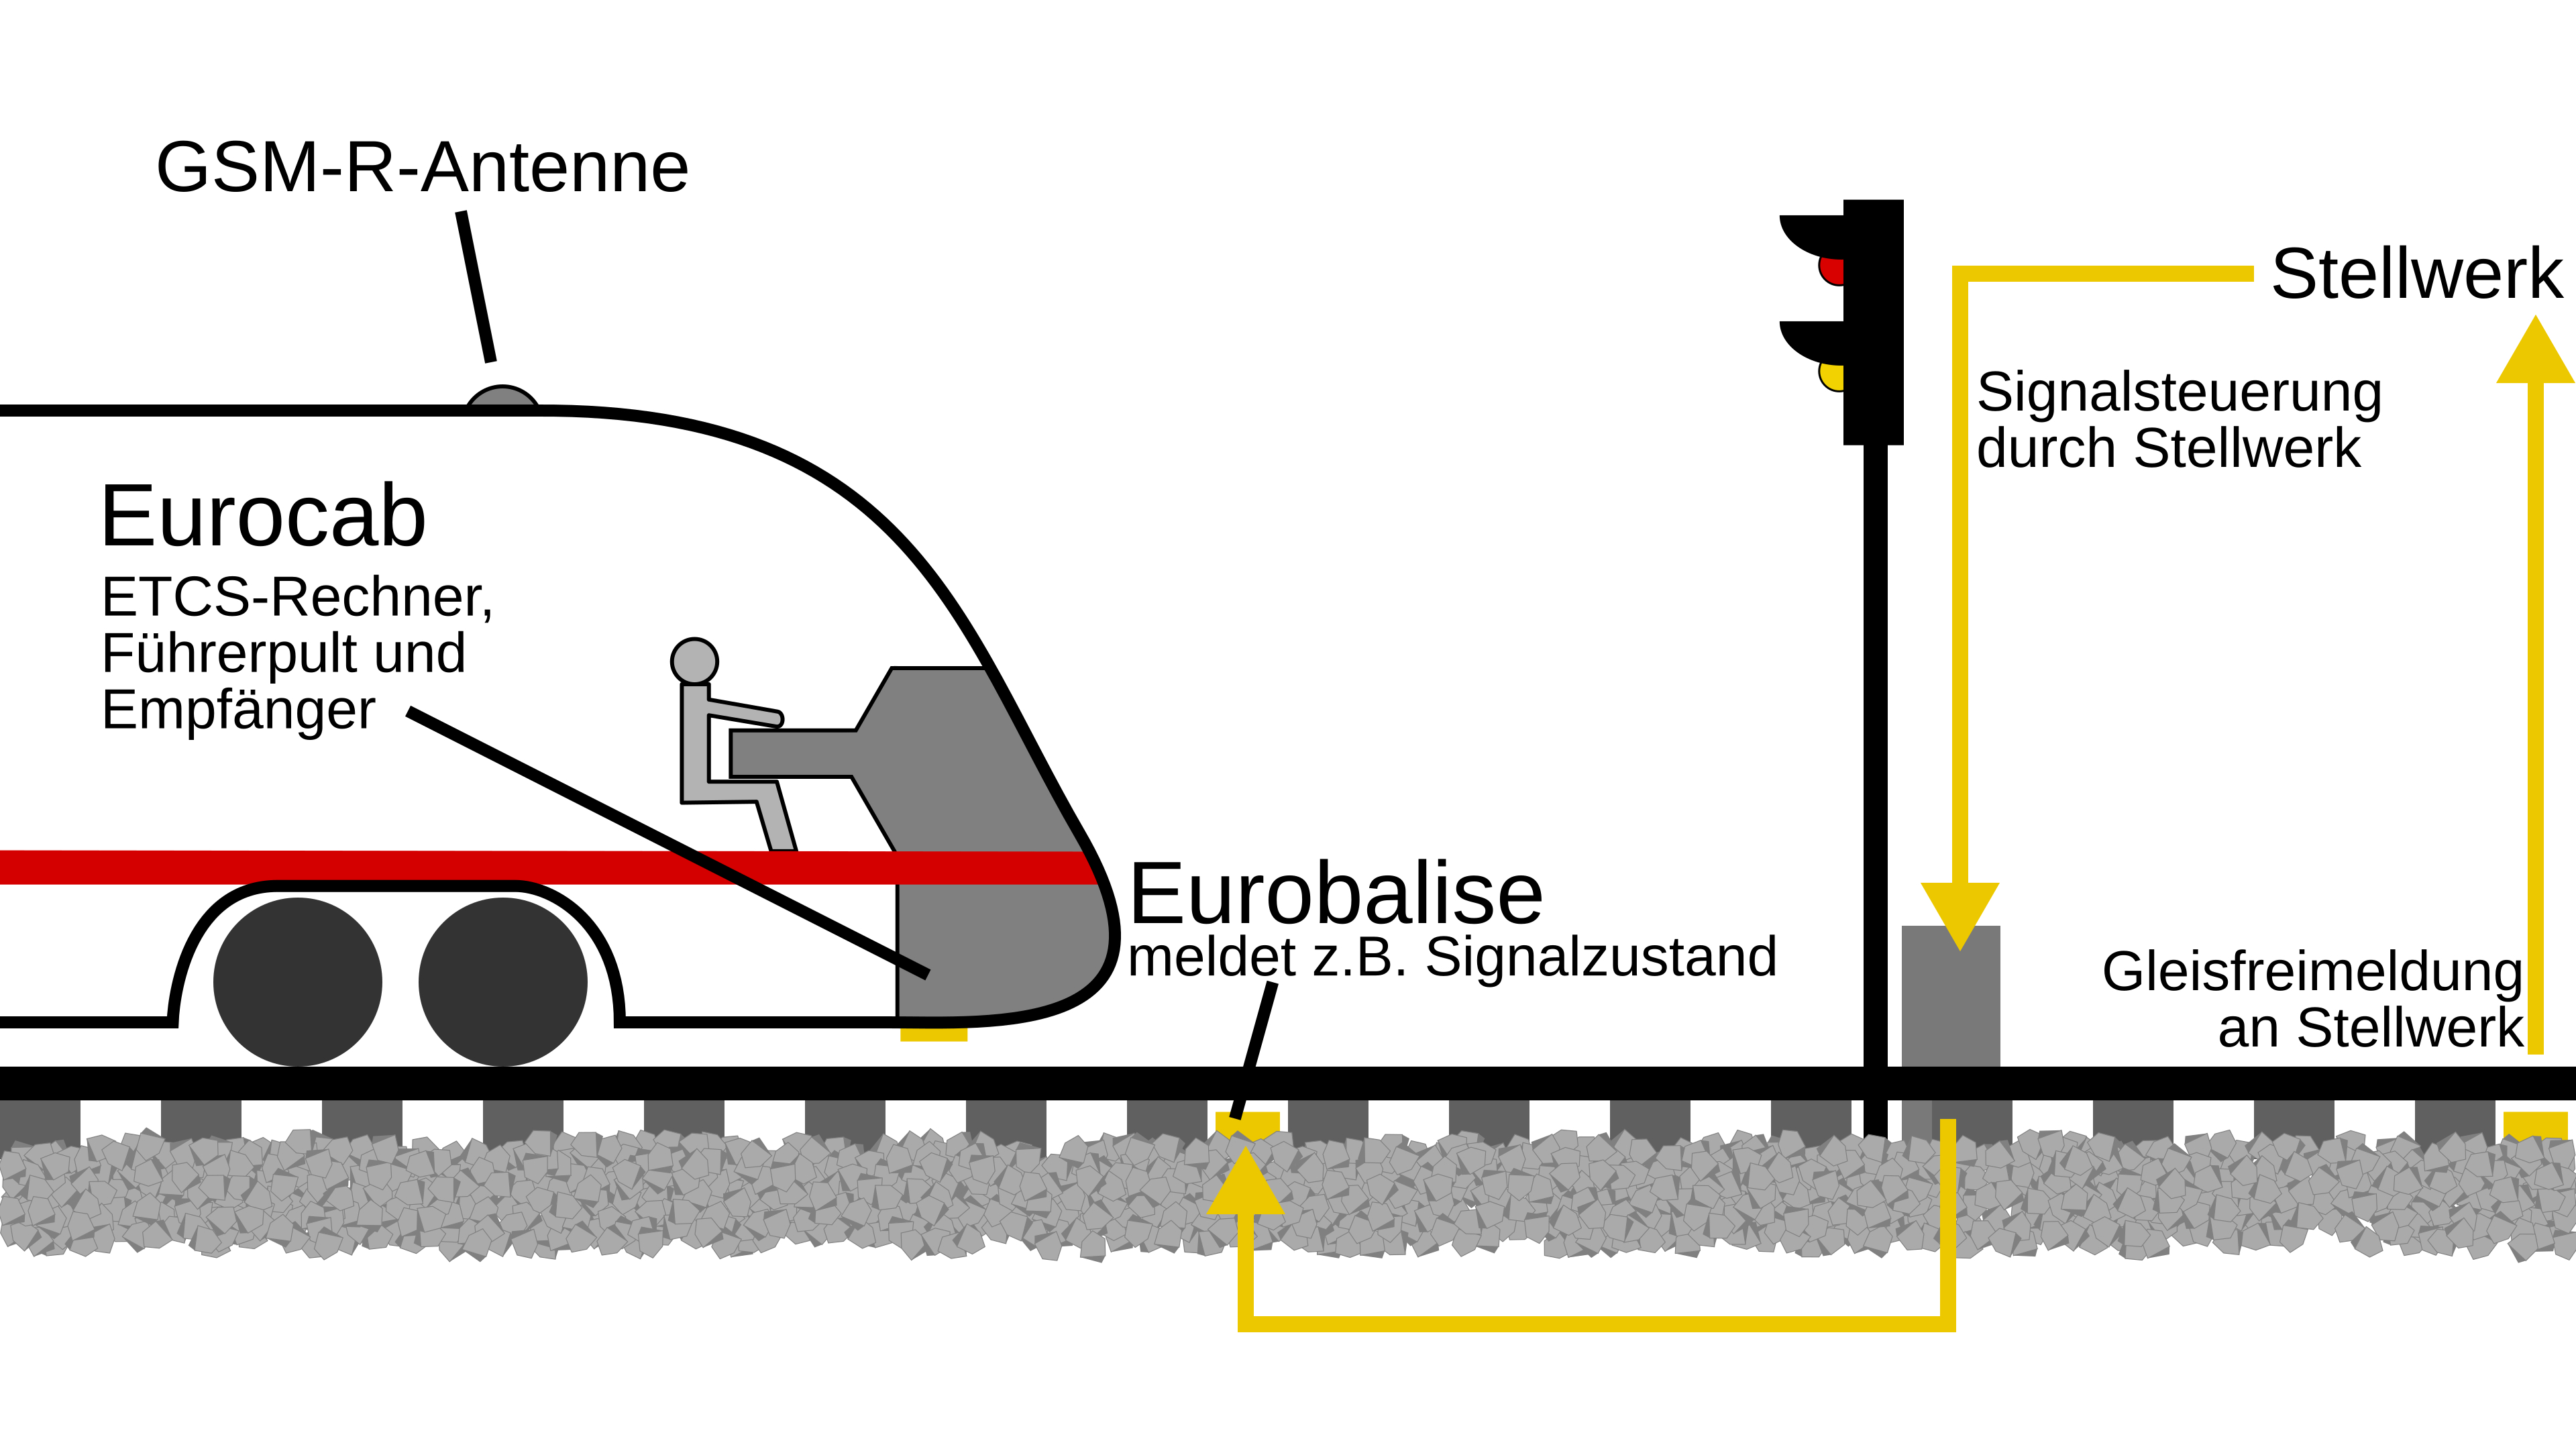
\includegraphics[width=0.65\textwidth]{res/ECTS_Level1.jpg}
    % \caption{\gls{etcs} \textit{Level} 1~\cite{sansculotteETCSLevel1}}
    % \label{fig:ETCS-level-1}
    % \end{figure}

    \item \textbf{\gls{etcs} \textit{Level} 1:} Funktioniert als punktförmiges System, das meist als \textit{Overlay} auf bestehenden nationalen Signalsystemen installiert wird. Fahrterlaubnisse (\textit{Movement Authorities}, \gls{ma}) werden von der Streckenzentrale über \textit{Lineside Equipment Units} (\gls{leu}) an Eurobalisen übertragen, die beim Überfahren vom fahrzeugseitigen Balisenleser (\gls{btm}) ausgelesen werden. Die Streckeneinteilung basiert auf festen Blockabschnitten~\parencite[S. 50, 71]{trinckaufETCS2024}~\parencite[S. 744]{chothiaAttack2017}.
    
    % \begin{figure}[htbp!]
    % \centering
    % 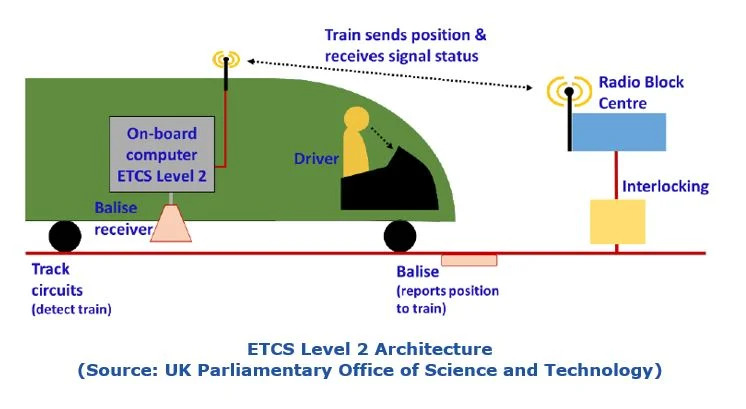
\includegraphics[width=0.65\textwidth]{res/ECTS_Level2.jpg}
    % \caption{\gls{etcs} \textit{Level} 2~\cite{arcETCS}}
    % \label{fig:ETCS-level-2}
    % \end{figure}
    
    \item \textbf{\gls{etcs} \textit{Level} 2:} Bietet eine kontinuierliche, funkbasierte Datenverbindung zwischen der fahrzeugseitigen \textit{On-Board-Unit} (\gls{obu}/\gls{evc}) und dem \textit{Radio Block Centre} (\gls{rbc}). Das \gls{rbc} verarbeitet Stellwerksinformationen sowie fahrzeugseitige Positionsberichte und generiert kontinuierlich \textit{Movement Authorities}, die per Funk an das Fahrzeug übertragen werden. Ortsfeste Signale an der Strecke sind technisch nicht mehr erforderlich~\parencite[S. 71, 89--90]{trinckaufETCS2024}.
    
    % \begin{figure}[H]
    % \centering
    % 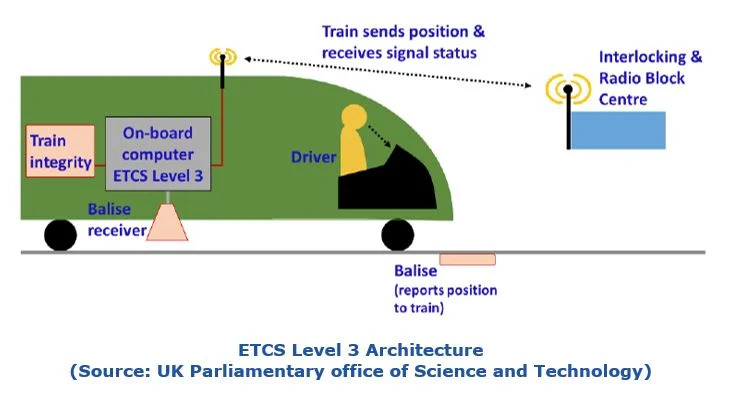
\includegraphics[width=0.65\textwidth]{res/ECTS_Level3.jpg}
    % \caption{\gls{etcs} \textit{Level} 3~\cite{arcETCS}}
    % \label{fig:ETCS-level-3}
    % \end{figure}

    \item \textbf{\gls{etcs} \textit{Level} 3:} Ersetzt gleisseitige Freimeldesysteme (wie Achszähler) durch eine kontinuierliche fahrzeugseitige Ortung und Integritätsüberprüfung (\textit{Train Integrity Monitoring System}, \gls{tims}). Dies ermöglicht den Betrieb im \textit{Moving Block} (gleitender Raumabstand), bei dem Züge auf Basis dynamischer Schutzabstände hintereinander fahren~\parencite[S. 471--472]{trinckaufETCS2024}~\parencite[S. 744]{chothiaAttack2017}.
\end{itemize}

% TODO add and Research more on this!: Aktuelle Lage! ETCS 3 ist am meisten noch in Testing bereich besonders wichitg für ATO-Entwicklung. Aber dien miesten Länder in Europa nutzt schon Level 1 einige versucht Lvl. 2 zu implementieren (RESEARCH: wo wurde implementiert, welche Bereiche/Strecke!)

\subsubsection{\texorpdfstring{Der \gls{ertms}-Kommunikationsstapel}{Der ERTMS-Kommunikationsstapel}}
\label{sec:Der_ERTMS-Kommunikationsstapel}
Die Kommunikation zwischen Zug und Radio Block Centre (RBC) ist in mehrere Protokollschichten gegliedert, die unterschiedliche Aufgaben bei Übertragung und Absicherung der ETCS-Daten übernehmen \parencite[S.744]{chothiaAttack2017}.

\begin{table}[ht]
\centering
\caption{Schichten des ERTMS-Kommunikationsstapels}
\label{tab:ertms-kommunikationsstapel}
\begin{tabularx}{\textwidth}{@{} X X X @{}}
\toprule
\textbf{Schicht} & \textbf{Technologie} & \textbf{Funktion} \\
\midrule
Untere Schicht
& GSM-R / RMR
& Übertragungsinfrastruktur zwischen Fahrzeug und Strecke; Schutz der
Funkschnittstelle, z.\,B. durch A5/1 oder A5/3
\parencite[S.744, 750]{chothiaAttack2017}. \\

Mittlere Schicht
& EuroRadio
& Authentifizierung und Integritätsschutz der ETCS-Daten mittels
Message Authentication Codes (MAC)
\parencite[S.744, 751]{chothiaAttack2017}. \\

Anwendungsschicht
& ETCS
& Verarbeitung betrieblicher Daten wie Movement Authorities und
Positionsberichte; Erkennung veralteter oder wiederholter Telegramme
durch Zeitstempel und Sequenznummern
\parencite[S.744, 754]{chothiaAttack2017}. \\
\bottomrule
\end{tabularx}
\end{table}

\subsubsection{\texorpdfstring{Nachfolgetechnologie \gls{rmr} und \gls{frmcs}}{Nachfolgetechnologie RMR und FRMCS}}
\label{sec:Nachfolgetechnologie_RMR_und_FRMCS}
Zur Ablösung der veraltenden \gls{2g}-basierten \gls{gsm-r}-Infrastruktur Spezifiziert die \gls{uic} im Rahmen des \textit{Railway Mobile Radio} (\gls{rmr}) das \textit{Future Railway Mobile Communication System} (\gls{frmcs}) als neuen globalen Mobilfunkstandard~\parencite[S. 49, 123]{trinckaufETCS2024}. Architektonisch basiert \gls{frmcs} auf den \gls{3gpp}-Spezifikationen (ab \textit{Release} 15/16) und führt ein dreischichtiges Architekturmodell ein, welches die Anwendungsschicht (\textit{Application Stratum}), die bahnspezifische Dienstschicht (\textit{Service Stratum} mit \gls{3gpp} \gls{mcx}-Diensten) und die physikalische Übertragungsschicht (\textit{Transport Stratum}) strikt voneinander entkoppelt~\parencite[S. 123]{trinckaufETCS2024}. 

Durch diese funktionale Entkopplung ist das System vollständig trägerunabhängig (\textit{Bearer Independence}): Die bahnbetriebliche Anwendungslogik und deren \textit{Safety}-Zertifikate werden von der zugrundeliegenden Übertragungsinfrastruktur isoliert~\parencite[S. 123, 211]{trinckaufETCS2024}. Dies ermöglicht es, zukünftige Mobilfunkgenerationen (wie \gls{6g}) oder alternative Übertragungsmedien (z. B. öffentliches \gls{5g}, \gls{wi-fi} oder Satellitenkommunikation) flexibel einzubinden, ohne dass die sicherheitskritische Zugsteuerungssoftware des \textit{European Vital Computers} (\gls{evc}) bei jedem Technologie-\textit{Upgrade} neu zertifiziert werden muss~\parencite[S. 123, 211]{trinckaufETCS2024}. Fahrzeugseitig stellt die \textit{Telecom On-Board Architecture} (\gls{toba}) über das \gls{frmcs} \textit{On-Board Gateway} und standardisierte Schnittstellen sicher, dass Funkmodule, Modems und Antennen modular ausgetauscht werden können, ohne die Trennung zwischen \textit{Safety} und \textit{Security} zu verletzen~\parencite[S. 123, 219]{trinckaufETCS2024}.

\subsubsection{\texorpdfstring{Kryptographische Schutzmechanismen und Schlüsselmanagement in \gls{etcs}}{Kryptographische Schutzmechanismen und Schlüsselmanagement in ETCS}}
\label{sec:Kryptographische_Schutzmechanismen_und_Schlüsselmanagement_in_ETCS}
Im traditionellen \textit{EuroRadio}-Protokoll erfolgt die Absicherung über den \textit{EuroRadio}-\gls{mac}-Algorithmus % TOLONG INI "mus"-nya harus turun kebawah, lihat PDF!
(eine Modifikation des \gls{iso} 9797-1 \gls{mac}-Algorithmus 3). Dieser berechnet einen 64-Bit-\gls{mac} mittels \gls{cbc}-Verfahren unter Nutzung von \textit{Single}-\gls{des} für die ersten $n-1$ Blöcke und \textit{Triple}-\gls{des} (\gls{3des}) für den finalen Block~\parencite[S. 751]{chothiaAttack2017}. Die Verwaltung der symmetrischen Sitzungsschlüssel (\gls{kmac}) obliegt einem hierarchischen \textit{Key Management System} (\gls{kms}) mit streckenseitigen \textit{Key Management Centren} (\gls{kmc})~\parencite[S. 90, 100]{trinckaufETCS2024}.

In neueren \gls{etcs}-Spezifikationen (ab \textit{Baseline} 4) wird die Absicherung der \textit{Euroradio}-Kommunikation auf eine \textit{End-to-End}-Verschlüsselung mittels \textit{Transport Layer Security} (\gls{tls}) umgestellt~\parencite[S. 211]{trinckaufETCS2024}. \gls{tls} stellt die Authentifizierung der Kommunikationspartner über \gls{x509}-Zertifikate innerhalb einer \textit{Public Key Infrastructure} (\gls{pki}) bereit und kapselt den gesamten Datenverkehr in einem kryptographisch gesicherten \gls{tcpip}-Tunnel~\parencite[S. 105, 211]{trinckaufETCS2024}.

\subsubsection{\texorpdfstring{Sichere \textit{Software}-Partitionierung: \gls{mils} und \textit{Separation Kernels}}{Sichere Software-Partitionierung: MILS und Separation Kernels}}
\label{sec:Sichere_Software-Partitionierung_MILS_und_Separation_Kernels}
Aufgrund der unterschiedlichen Lebenszyklen von \textit{Safety}-Anwendungen (ca. 20 Jahre) und \textit{Security}-Protokollen (ca. 2--5 Jahre) wird in modernen Fahrzeuggeräten das \gls{mils}-Architekturmuster (\textit{Multiple Independent Levels of Security}) eingesetzt~\parencite[S. 31--32]{schulzIntegration2019}~\parencite[S. 80--81]{tverdyshevCertMILS2019}. 

Ein zertifizierter \textit{Separation Kernel} (z. B. \textit{PikeOS}) unterteilt die Hardwareressourcen in strikt isolierte Partitionen. Dadurch läuft die sicherheitszertifizierte Steuerungslogik (z. B. \gls{scade}-Modelle) getrennt von der Kommunikations-\textit{Middleware} (z. B. \gls{trdp}) und dem Verschlüsselungstunnel (z. B. \textit{WireGuard} oder \gls{tls})~\parencite[S. 32--34]{schulzIntegration2019}. Dies ermöglicht eine modulare ("kompositionelle") Zertifizierung, bei der \textit{Security}-\textit{Updates} für Funktreiber eingespielt werden können, ohne den \textit{Safety}-Sicherheitsnachweis des Fahrzeugrechners zu invalidieren~\parencite[S. 31, 35]{schulzIntegration2019}~\parencite[S. 83]{tverdyshevCertMILS2019}.

\subsubsection{\texorpdfstring{Industrielle \gls{it}-Sicherheit nach \gls{iec} 62443 in der \gls{lst}}{Industrielle IT-Sicherheit nach IEC 62443 in der LST}}
\label{sec:Industrielle_IT-Sicherheit_nach_IEC_62443_in_der_LST}
Für die \gls{it}-Sicherheit ortsfester Leit- und Sicherungstechnikanlagen (\gls{lst}) findet der Standard \gls{iec} 62443 Anwendung~\parencite[S. 31, 33]{schulzIntegration2019}.
% \parencite[S. 41]{h.tsukisawaStandardization2024}. 
Er teilt das Gesamtsystem in Sicherheitszonen (\textit{Zones}) und logische Kommunikationskanäle \textit{Conduits} ein. An den Zonengrenzen überwachen \textit{Firewalls} und \textit{Security Gateways} den Datenfluss, um unbefugte Seitwärtsbewegungen \textit{Lateral Movement} zwischen betrieblichen Netzen und der Sicherungstechnik zu verhindern~\parencite[S. 33]{schulzIntegration2019}~\parencite[S. 43]{h.tsukisawaStandardization2024}. % FUTURE_DO: if there are places, PRIO1: Research and edit: yes it has zones and stuff, but I want more explanation from the ETCS in Deutschland. That maye more suitable to this subsection

% \subsubsection{Historische Basis: Altsignalisierung und mechanische Stellwerke}
% Die historische Basis der Streckensicherung bildet die fahrwegsicherungsphysische Abhängigkeit. In mechanischen Stellwerken wird die Zulässigkeit einer Zugfahrt durch ein Netzwerk aus mechanischen Hebeln, Verschlussregistern und Drahtzugleitungen erzwungen, welche die Einstellung kollidierender Fahrstraßen physisch verhindern \parencite[S. 239, 241]{Why trains don't usually crash into each other}. Das zugrundeliegende Sicherungsprinzip ist der feste Raumabstand (Absolute Block Principle), bei dem sich in jedem Blockabschnitt zu jedem Zeitpunkt nur ein einziger Zug befinden darf \parencite[S. 246--247]{Why trains don me usually crash into each other}. %FUTURE_DO: needs to be researched more ont his topic really! % NOTE: the thing is this why trains don't usually crash each other is basically a youtube Video. it could be COMMENT OUT!

\subsection{Japanische Eisenbahnarchitektur}
\label{sec:Japanische_Eisenbahnarchitektur}

\subsubsection{Historische Entwicklung und betreiberspezifische Heterogenität}
\label{sec:Historische_Entwicklung_und_betreiberspezifische_Heterogenität}
Die japanische Eisenbahninfrastruktur ist durch die Privatisierung der \textit{Japan National Railways} (\gls{jnr}) im Jahr 1987 geprägt, aus der mehrere unabhängig agierende regionale \gls{jr}-Gesellschaften (z. B. \gls{jr} \textit{East}, \gls{jr} \textit{Central}) sowie private Bahnbetreiber hervorgingen~\parencite[S. 47]{yanaseJapanese2011}. Während die Regierung minimale nationale Rahmenbestimmungen \textit{Technical Standards} vorgab, erhielten die Betreiber die Autonomie, eigene technische Implementierungsstandards \textit{Implementation Standards} zu entwickeln~\parencite[S. 48--49, 51]{yanaseJapanese2011}. Dies führte zu einer ausgeprägten regionalen und technischen Heterogenität der Signal- und Zugsicherungssysteme.

% Der Shinkansen wurde dabei von Beginn an als physisch und betrieblich isoliertes Hochgeschwindigkeitssystem auf Normalspur (1.435 mm) konzipiert, das keine kreuzenden Bahnübergänge aufweist und vollständig vom schmalspurigen Bestandsnetz (1.067 mm) getrennt ist \parencite[S. 50]{yanaseJapanese2011} % NOT THAT IMPORTANT FOR MY HAUSARBEIT. THE MOST IMPORATNT IS THE TECHNISCHEN ISOLIERUNG AUF KOMMUNIKATIONSSYSTEM EBENE

\subsubsection{\texorpdfstring{\gls{atc} und \gls{atacs}}{ATC und ATACS}}
\label{sec:ATC_und_ATACS}
Die Signaltechnik entwickelten die japanischen Betreiber von analogen \gls{atc}-Systemen (\textit{Automatic Train Control}) hin zu digitalen Funksteuerungssystemen weiter:

\begin{itemize}
    \item \textbf{\textit{Digital} \gls{atc} (\gls{d-atc}):} Nutzt codierte Schienenstromkreise zur Übertragung digitaler Telegramme an das Fahrzeug. Die \gls{obu} berechnet anhand der empfangenen Zielentfernung kontinuierliche Bremskurven~\parencite[S. 44--45]{h.tsukisawaStandardization2024}.
    \item \textbf{\gls{atacs} (\textit{Advanced Train Administration and Communications System}):} Ein von \gls{jr} \textit{East} entwickeltes funkbasiertes Zugsteuerungssystem~\parencite[S. 13--14]{xiangliuCyber2020}~\parencite[S. 45]{h.tsukisawaStandardization2024}. Im Gegensatz zu \gls{etcs} \textit{Level} 2 ermittelt der Zug seine Position eigenständig über Radsensoren und Gleis-\textit{Transponder} und sendet diese \textit{via} \gls{tdma}-Funk (\textit{Time Division Multiple Access}) oder \textit{Leaky-Coaxial}-Kabel (\gls{lcx}) an die Erfassungsrechner~\parencite[S. 6, 8]{iwamotoTrain2024}~\parencite[S. 14]{xiangliuCyber2020}. \gls{atacs} nutzt eine dezentrale Logikstruktur (\textit{Decentralized Traffic Control}) zur Erzeugung dynamischer Bremskurven im \textit{Moving Block}~\parencite[S. 14]{xiangliuCyber2020}.
\end{itemize}

\subsubsection{\texorpdfstring{Unabhängige Zugsteuerung und \gls{iec} 62280}{Unabhängige Zugsteuerung und IEC 62280}}
\label{sec:Unabhängige_Zugsteuerung_und_IEC_62280}
Aktuelle Forschungen des \textit{Railway Technical Research Institute} (\gls{rtri}) adressieren die hohen Bau- und Wartungskosten privater Funknetze (\gls{lcx}) durch das Konzept der \textbf{Unabhängigen Zugsteuerung} (\textit{Train Control System Independent of Communication Transmission Paths})~\parencite[S. 1--3]{iwamotoTrain2024}. 

Das Kernprinzip basiert auf der strikten funktionalen Trennung von Sicherheitssteuerungsfunktionen und Informationsübertragungsfunktionen~\parencite[S. 1, 4]{iwamotoTrain2024}. Zur Behandlung der sieben Übertragungsbedrohungen nach der Schnittstellennorm \gls{iec} 62280 (Wiederholung, Löschung, Einfügung, Änderung der Reihenfolge, Verfälschung, Verzögerung, Identitätsfälschung) wird das Steuerungskonzept in zwei Modelle unterteilt~\parencite[S. 7, 10--11]{iwamotoTrain2024}:

\begin{itemize}
    \item \textbf{Sicherheitsbestätigende Steuerung (\textit{Safety Confirmation-type Control}):} Wird für die Erteilung von Fahrterlaubnissen genutzt. Das Fahrzeug darf nur weiterfahren, wenn explizite, positiv verifizierte Steuerungsdaten empfangen werden~\parencite[S. 10--11]{iwamotoTrain2024}.
    
    \item \textbf{Gefahrenerkennende Steuerung (\textit{Danger Detection-type Control}):} Wird für hochpriorisierte Notstopps genutzt. Sie erfordert eine hochfrequente, zyklische Datenübertragung; bleibt diese über ein definiertes Zeitfenster aus, leitet das Fahrzeug automatisch einen Notstopp ein~\parencite[S. 10--12]{iwamotoTrain2024}.
\end{itemize}

Diese Trennung ermöglicht es, öffentliche Mobilfunknetze (\gls{5g}) oder \gls{wi-fi} als Übertragungsmedien einzusetzen, da die Integrität der Sicherheitslogik auf Protokollebene verifiziert wird~\parencite[S. 3, 10]{iwamotoTrain2024}.

\subsubsection{Kryptographische Absicherung in Japan}
\label{sec:Kryptographische_Absicherung_in_Japan}
Im Rahmen des \gls{rtri}-Ansatzes wird zur Fälschungssicherung 
%(なりすまし) % Text type -- Hiragana -- Somehow not supported!
ein \textit{Hash-based Message Authentication Code} auf Basis von \gls{sha-256} (\textbf{\gls{hmac-sha256}}) eingesetzt~\parencite[S. 12]{iwamotoTrain2024}. Gemäß den \gls{cryptrec}-Standards bietet \gls{hmac-sha256} eine kryptographische Sicherheitsstärke von 256 Bit, die bis mindestens zum Jahr 2070 als mathematisch robust eingestuft wird~\parencite[S. 12]{iwamotoTrain2024}. 

Da japanische Bahnbetreiber als private Unternehmen agieren, sind konkrete Details zur Schlüsselverwaltung (\textit{Key Management}) sowie zu den operativen Schnittstellen des Kryptomoduls in öffentlich zugänglichen wissenschaftlichen Quellen nicht im Detail dokumentiert~\parencite[S. 47]{yanaseJapanese2011}.


\section{Methodik}
\label{sec:Methodik}

\subsection{Forschungsdesign: Strukturierte Literaturanalyse}
\label{sec:Forschungsdesign_Strukturierte_Literaturanalyse}

Diese Hausarbeit basiert auf einer strukturierten Literaturanalyse. Hierfür werden technische Standards, offizielle Dokumentationen, wissenschaftliche Veröffentlichungen sowie ausgewählte Branchenberichte zur sicherheitskritischen Eisenbahnkommunikation ausgewertet. Aufgrund der sicherheitskritischen Natur von Zugsteuerungssystemen sowie der rechtlichen und betrieblichen Risiken wären direkte Penetrationstests oder experimentelle Manipulationen realer Eisenbahninfrastruktur im Rahmen dieser Arbeit unangemessen~\cite{Chothia2017}.

Ziel der Analyse ist nicht die vollständige technische Beschreibung einzelner Eisenbahnsysteme, sondern die vergleichende Untersuchung zentraler architektonischer und sicherheitsbezogener Prinzipien der Zug-Strecken-Kommunikation.

\subsection{Vergleichsrahmen und Einschränkungen}
\label{sec:Vergleichsrahmen_und_Einschränkungen}

Der Vergleich konzentriert sich auf sicherheitskritische Kommunikationsschnittstellen europäischer und japanischer Eisenbahnsysteme, insbesondere zwischen Fahrzeugen und streckenseitigen beziehungsweise zentralen Steuerungskomponenten. Betrachtet werden dabei die Übertragung sicherheitsrelevanter Informationen wie \textit{Movement Authorities}, Positionsmeldungen und Geschwindigkeitsinformationen. Für Europa stehen \gls{ertms}, \gls{etcs}, \gls{gsm-r}, \textit{EuroRadio} sowie die Migration zu \gls{frmcs} im Mittelpunkt; für Japan werden ausgewählte Zugsteuerungs- und Kommunikationssysteme sowie aktuelle Forschungsansätze zur funkbasierten Zugsteuerung untersucht.

Die Analyse basiert ausschließlich auf öffentlich verfügbarer Literatur. Konkrete Implementierungsdetails, Netzwerktopologien und Sicherheitskonfigurationen einzelner Betreiber sind daher nur eingeschränkt zugänglich. Zudem werden weder sämtliche europäischen Eisenbahnsysteme noch alle japanischen Betreiber betrachtet. Fahrgast-\gls{wlan}, Fahrgastinformationssysteme, \textit{Ticketing} und allgemeine Unternehmens-\gls{it} liegen außerhalb des Untersuchungsumfangs. Da sowohl etablierte Systeme als auch Forschungs- und Migrationsansätze einbezogen werden, erfolgt die Untersuchung als architektonischer und literaturbasierter Vergleich und nicht als empirische Sicherheitsprüfung konkreter Infrastrukturen.

\subsection{Bewertungsverfahren}
\label{sec:Bewertungsverfahren}

Die Literatur wird in vier Schritten ausgewertet:

\begin{enumerate}
    \item \textbf{Kommunikationsarchitekturen:} Identifikation der für die Zug-Strecken-Kommunikation relevanten Systeme und Schnittstellen auf Grundlage des in Kapitel 2 dargestellten Bezugsrahmens.

    \item \textbf{Bedrohungen:} Erfassung relevanter Angriffsmöglichkeiten wie Nachrichtenmanipulation, \textit{Replay}, Fälschung, \textit{Jamming}, \textit{Denial-of-Service} und Angriffe auf streckenseitige Komponenten.

    \item \textbf{Sicherheitsmechanismen:} Analyse technischer und architektonischer Schutzmaßnahmen, insbesondere Authentifizierung, Integritätsschutz, Fehlererkennung und funktionale Trennung sicherheitskritischer Funktionen vom Übertragungsmedium.

    \item \textbf{Vergleichende Bewertung:} Gegenüberstellung der Systeme hinsichtlich Gemeinsamkeiten, Unterschieden, Sicherheitsgrenzen sowie Evidenz- und Forschungslücken.
\end{enumerate}

\section{Diskussion}
\label{sec:Diskussion}

\subsection{\texorpdfstring{\gls{etcs}-\textit{Level}-Vergleich: Operative, humane und kommunikative Schnittstellen}{ETCS-Level-Vergleich: Operative, humane und kommunikative Schnittstellen}}
\label{sec:ETCS-Level-Vergleich_Operative_humane_und_kommunikative_Schnittstellen}
Die Weiterentwicklung der europäischen Zugsicherung vollzieht sich in einer klaren Differenzierung zwischen der Kommunikationsarchitektur (\gls{etcs}-\textit{Level}) und dem standardisierten Funktionsstand (\textit{Baseline} und Systemversion)~\parencite[S. 50--53]{trinckaufETCS2024}. Dieser Ebenentrennung liegen spezifische Vor- und Nachteile auf operativer, humaner und kommunikativer Ebene zugrunde:

\begin{itemize}
    \item \textbf{\gls{etcs} \textit{Level} 1 (Punktförmig):} Bietet den Vorteil einer unkomplizierten \textit{Overlay}-Installation auf bestehenden Signalanlagen ohne hohe Anforderungen an das Funknetz~\parencite[S. 71]{trinckaufETCS2024}. Auf humaner und operativer Seite entsteht jedoch eine hohe Belastung für das Fahrpersonal, da ortsfeste Lichtsignale weiterhin parallel zur Führerraumsignalisierung beobachtet werden müssen. Zudem erfolgen Aktualisierungen der Fahrterlaubnis (\textit{Movement Authority}, \gls{ma}) nur diskret beim Überfahren von Eurobalisen, was die Streckenkapazität einschränkt (siehe \autoref{sec:Struktur_und_Funktionsweise}).
    \item \textbf{\gls{etcs} \textit{Level} 2 (Kontinuierlich, funkbasiert):} Erlaubt den vollständigen Entfall ortsfester Signale (\gls{l2os}) und entlastet den Triebfahrzeugführer durch kontinuierliche, dynamische Bremskurvenüberwachung im \textit{Driver Machine Interface} (\gls{dmi})~\parencite[S. 89--90]{trinckaufETCS2024}. Die Schattenseite liegt in der strikten Abhängigkeit von der Funkübertragung (\gls{gsm-r}/\gls{rbc}): Fällt die Verbindung abseits definierter Toleranzzeiten aus, erzwingt die Sicherheitslogik im Sinne des \textit{Fail-Safe}-Prinzips (\textit{Intrinsic Safety}) den sofortigen Zughalt, was das System anfällig für betriebliche Stillstände macht (siehe \autoref{sec:Sicherheitskritische_Eisenbahnkommunikation}).
    \item \textbf{\gls{etcs} \textit{Level} 3 (\textit{Moving Block} / \gls{tims}):} Maximiert die Streckenkapazität durch den Verzicht auf gleisseitige Freimeldeanlagen~\parencite[S. 471--472]{trinckaufETCS2024}. Die zentrale Schwachstelle ist hierbei die humane und technische Komplexität der fahrzeugseitigen Zugintegritätsüberwachung (\gls{tims}) – insbesondere im Güterverkehr –, da fehlerhafte \textit{Timer}-Abgleiche zu fälschlichen Blockblockaden („Schattenzüge“) führen können.
\end{itemize}

Das Zusammenspiel von \textit{Baselines} und Systemversionen (z. B. \textit{Baseline} 4 mit Systemversion 3.0) löst das Spannungsfeld zwischen Innovation und Kontinuität: Neue Funktionen (wie \gls{ato} oder \gls{frmcs}-Schnittstellen) können gezielt integriert und Fehler über bindende \textit{Change Requests} korrigiert werden, während Abwärtskompatibilität und Versionsmanagement die grenzüberschreitende Interoperabilität sichern~\parencite[S. 53, 218--220]{trinckaufETCS2024}.

\subsection{Sicherheitsarchitektur: Interoperabilität \textit{vs.} Betreiberspezifische Diversität}
\label{sec:Sicherheitsarchitektur_Interoperabilität_vs_Betreiberspezifische_Diversität}
Der Vergleich der europäischen und japanischen Sicherheitsarchitekturen offenbart zwei grundlegend unterschiedliche Designphilosophien:

Europas Stärke liegt in der völkerrechtlich und technisch garantierten Interoperabilität auf Basis der \gls{tsiccs}~\parencite[S. 49]{trinckaufETCS2024}. Der Preis dieser Standardisierung ist jedoch das Verharren von Altsystemen (\textit{Legacy Security}): Da Schnittstellen über Jahrzehnte abwärtskompatibel bleiben müssen, bleiben veraltete Protokolle wie \gls{gsm-r} und \textit{EuroRadio} trotz bekannter Sicherheitsmängel im Netz gebunden (siehe \autoref{sec:Japanische_Eisenbahnarchitektur}). Um dieser Obsoleszenz zu begegnen, adressiert Europa die logische Trennung von Anwendungs- und Übertragungsschicht durch die schrittweise Migration zum \textit{Future Railway Mobile Communication System} (\gls{frmcs}) im Rahmen von \gls{rmr}, das eine trägerunabhängige Kommunikation über \gls{5g}- und \gls{ip}-Netze ermöglicht~\parencite[S. 123, 211]{trinckaufETCS2024}.

In Japan führte die Privatisierung der \gls{jnr} hingegen zu einer ausgeprägten betreiberspezifischen Heterogenität~\parencite[S. 47--49]{yanaseJapanese2011}. Aus \textit{Security}-Perspektive erzeugt diese Struktur ein inhärentes Schutzkonzept durch Systemdiversität (\textit{Security through Diversity}): Wird eine herstellerspezifische Implementierung (z. B. \gls{atacs} bei \gls{jr} \textit{East}) kompromittiert, breitet sich der Angriff nicht automatisch auf andere regionale Betreiber oder das isolierte \textit{Shinkansen}-Netz aus. Der operative Nachteil liegt jedoch in einer immensen Management- und Zertifizierungskomplexität (\textit{Security-Management Complexity}) sowie dem Fehlen skalenbedingter Kostenvorteile beim Hardwarebezug.

Parallel dazu markiert die japanische Forschung zur \textbf{Unabhängigen Zugsteuerung} (\gls{rtri}) einen vergleichbaren Paradigmenwechsel~\parencite[S. 1--3]{iwamotoTrain2024}. Statt sich wie historisch auf physisch isolierte Sondernetze (\gls{lcx}-Kabel) zu verlassen, behandelt dieser Ansatz das Übertragungsmedium als potenziell ungesichert (\textit{Untrusted Conduit}) gemäß \gls{iec} 62280. Die Schutzfunktion wird von der physischen Infrastruktur vollständig auf die Logikschicht verlagert, wo Nachrichten mittels \gls{hmac-sha256} kryptographisch authentifiziert werden (siehe \autoref{sec:Kryptographische_Absicherung_in_Japan}).

\subsection{\texorpdfstring{Kryptographische Schwachstellen und \gls{mils}-basierte Architekturkapselung}{Kryptographische Schwachstellen und MILS-basierte Architekturkapselung}}
\label{sec:Kryptographische_Schwachstellen_und_MILS-basierte_Architekturkapselung}
Die Notwendigkeit einer logischen Entkopplung wird durch die kryptographischen Schwachstellen klassischer Bahnfunkprotokolle untermauert. Der \textit{EuroRadio}-\gls{mac} basiert auf einer modifizierten 64-Bit-\gls{cbc}-Konstruktion aus \textit{Single}-\gls{des} und \textit{Triple}-\gls{des}~\parencite[S. 751]{chothiaAttack2017}. Wie Chothia \textit{et al.} nachweisen, erlaubt die begrenzte Blocklänge kollisionsbasierte Angriffe: Durch das Beobachten von Nachrichtenkollisionen kann ein Angreifer den ersten \gls{des}-Schlüssel ($k_1$) mathematisch gewinnen und anschließend gefälschte \textit{Movement Authorities} (z. B. versteckt im unüberwachten Paket) in den Datenstrom injizieren~\parencite[S. 751--754]{chothiaAttack2017}.

An dieser Stelle setzt das \gls{mils}-Architekturmuster (\textit{Multiple Independent Levels of Security}) an, um das Gesamtsystem trotz potenzieller Kommunikationsschwachstellen zu schützen (siehe \autoref{sec:Sichere_Software-Partitionierung_MILS_und_Separation_Kernels})~\parencite[S. 31--32]{schulzIntegration2019}:

\begin{enumerate}
    \item \textbf{Schutz vor Privilegienerweiterung und Durchgreifen:} Ein zertifizierter \textit{Separation Kernel} unterteilt den Fahrzeugrechner (\gls{evc}) in strikt isolierte \textit{Hardware}-Partitionen. Selbst wenn ein Angreifer Schwachstellen im \gls{gsm-r}-Modem, im Protokollstapel oder bei der Schlüsselverwaltung (\gls{kmc}) ausnutzt, verhindert die \gls{mils}-Isolierung ein Ausbrechen des Angreifers auf die sicherheitskritische Steuerungsebene (\textit{Safety-Logic})~\parencite[S. 32--34]{schulzIntegration2019}~\parencite[S. 80--81]{tverdyshevCertMILS2019}.
    \item \textbf{Entkopplung der Lebenszyklen:} \gls{mils} ermöglicht eine kompositionelle Zertifizierung. Kryptographische Protokolle oder Funktreiber (mit Lebenszyklen von 2--5 Jahren) können aktualisiert und gepatcht werden, ohne dass der \textit{Safety}-Sicherheitsnachweis der Kernsteuerungssoftware (mit Lebenszyklen von über 20 Jahren) invalidiert wird~\parencite[S. 31, 35]{schulzIntegration2019}~\parencite[S. 83]{tverdyshevCertMILS2019}.
\end{enumerate}

\subsection{\texorpdfstring{\gls{ids}, \gls{mtd} und Redundanzkonzepte}{IDS, MTD und Redundanzkonzepte}}
\label{sec:IDS_MTD_und_Redundanzkonzepte}
Zur Absicherung gegen Angriffe auf Netzwerkechzeit und Verfügbarkeit genügen rein kryptographische Verfahren nicht. Daher werden ergänzende Abwehrmechanismen diskutiert:

\begin{itemize}
    \item \textbf{\textit{Moving Target Defense} (\gls{mtd}):} Verfahren wie \textit{Port Hopping} oder \gls{ip}-\textit{Address Shuffling} erschweren gegnerische Netzwerk-\textit{Scans}~\parencite[S. 121]{poschingerOpenMTD2020}. Im Eisenbahnumfeld muss \gls{mtd} jedoch mit extremer Zurückhaltung eingesetzt werden. Sicherheitskritische Funktelegramme besitzen mikrosekundengenaue \textit{Timing}-Anforderungen. Zusätzliche Latenzen, Synchronisationsfehler oder Paketverluste durch Adress-\textit{Swaps} sind im \gls{lst}-Bereich inakzeptabel. \gls{mtd} eignet sich daher primär als komplementärer Schutz für nachgelagerte, nicht-zeitkritische Managementschnittstellen~\parencite[S. 121]{poschingerOpenMTD2020}.
    \item \textbf{\textit{Intrusion Detection Systems} (\gls{ids}):} Systeme wie \gls{rrids} vergleichen empfangene Funkverläufe passiv mit mathematischen Soll-Zustandsmodellen (\gls{mutesla}) und identifizieren \textit{Replay}- oder \textit{Jamming}-Versuche echtzeitnah, ohne Latenzen in den Steuerungszirkel einzubringen~\parencite[S. 60--63]{melaragnoRail2016}.
\end{itemize}

Bezüglich der \textbf{Verfügbarkeit} zeigen sich deutliche Unterschiede im Redundanzdesign: Während traditionelle japanische Systeme auf physische Doppelung (z. B. redundante \gls{lcx}-Kabelstränge entlang der Trasse) setzten~\parencite[S. 14--15]{xiangliuCyber2020}, baut Europa im Rahmen der Digitalen Schiene Deutschland auf räumliche Funknetzredundanz und redundante \gls{rbc}-Zentren (z. B. im Knoten Stuttgart/Ulm)~\parencite[S. 89--90, 211]{trinckaufETCS2024}. Wie reale Großstörungen jedoch belegen, schützt reine \textit{Hardware}-Redundanz nicht vor zentralen logischen Fehlerquellen (\textit{Single Point of Failure}, \gls{spof}) in den Vermittlungsschichten (z. B. \gls{hlr}- oder \textit{Switch}-Ausfälle im Kernnetz), die trotz vorhandener Reserven zur flächendeckenden Abschaltung des Zugfunks führen können.

\subsection{\texorpdfstring{Zukunftsfähige Migrationspfade: \gls{frmcs} und \gls{iec} 62280}{Zukunftsfähige Migrationspfade: FRMCS und IEC 62280}}
\label{sec:Zukunftsfähige_Migrationspfade_FRMCS_und_IEC_62280}
Die Überwindung der \gls{gsm-r}-Schwachstellen vollzieht sich in Europa durch die Migration zu \gls{frmcs} im Rahmen von \gls{rmr}~\parencite[S. 49, 123]{trinckaufETCS2024}. \gls{frmcs} eliminiert die Schwachstellen des \textit{EuroRadio}-\gls{mac}s, indem die Datenübertragung auf moderne \gls{tls}-1.3-Verschlüsselung mit \gls{pki}-Zertifikaten umgestellt wird~\parencite[S. 105, 211]{trinckaufETCS2024}. 

Überdies schützt die in \gls{frmcs} integrierte \textbf{\textit{Multipath}-Funktionalität} (parallele Bündelung von \gls{rmr}-\gls{5g} und öffentlichen Mobilfunknetzen) effektiv vor Breitband-\textit{Jamming} und stellt die erforderliche Bandbreite und Ausfallsicherheit für hochautomatisierten Betrieb (\gls{goa4}) bereit~\parencite[S. 123, 211]{trinckaufETCS2024}. Durch das trägerunabhängige Dreischichtenmodell (\textit{Application, Service, Transport Stratum}) können zukünftige Mobilfunkgenerationen (wie \gls{6g}) eingebunden werden, ohne die zertifizierte \gls{etcs}-Anwendungslogik zu verändern (siehe \autoref{sec:Nachfolgetechnologie_RMR_und_FRMCS}).

\subsection{Vergleichende Synthese}
\label{sec:Vergleichende_Synthese}

Der Vergleich zeigt unterschiedliche Ausgangspunkte bei zugleich ähnlicher Entwicklungsrichtung. Europa verfolgt mit \gls{ertms} einen stark standardisierten und interoperablen Ansatz, während die japanische Systemlandschaft stärker betreiber- und streckenspezifisch geprägt ist. Trotz dieser Unterschiede ist eine gemeinsame architektonische Tendenz erkennbar: Sowohl \gls{frmcs} als auch der untersuchte \gls{rtri}-Ansatz lösen sicherheitskritische Steuerungsfunktionen zunehmend vom konkreten Übertragungsmedium. Dadurch werden \textit{Safety}-Funktionen, \textit{Security}-Mechanismen und Kommunikationsinfrastruktur stärker funktional entkoppelt.

Eine vollständige Gleichsetzung beider Ansätze ist jedoch nicht möglich. \gls{frmcs} bildet einen standardisierten europäischen Migrationsrahmen, während die unabhängige Zugsteuerung des \gls{rtri} einen aktuellen Forschungsansatz darstellt. Zudem sind konkrete \textit{Security}-Implementierungen japanischer Betreiber öffentlich nur eingeschränkt dokumentiert, wodurch ein direkter Vergleich einzelner Sicherheitsmechanismen begrenzt bleibt.

\section{Fazit}
\label{sec:Fazit}

Die Untersuchung zeigt, dass europäische und japanische Eisenbahnsysteme sicherheitskritische Kommunikation mit unterschiedlichen architektonischen Ansätzen schützen. Europa setzt mit \gls{ertms} stärker auf Standardisierung und Interoperabilität, während Japan durch betreiber- und streckenspezifische Systeme geprägt ist. Gemeinsam ist beiden Ansätzen jedoch die zunehmende funktionale Trennung zwischen sicherheitskritischer Steuerungslogik und dem verwendeten Kommunikationsmedium.

Die Forschungsfrage lässt sich dahingehend beantworten, dass kryptographischer Integritäts- und Authentizitätsschutz zwar Manipulationen erschwert, die Verfügbarkeit der Kommunikation jedoch eine zentrale Sicherheitsgrenze bleibt. Kommunikationsstörungen können aufgrund des \textit{Fail-Safe}-Prinzips einen sicheren Zustand erzwingen, gleichzeitig aber erhebliche betriebliche Einschränkungen verursachen.

Eine abschließende Bewertung wird insbesondere durch die begrenzte öffentliche Dokumentation konkreter \textit{Security}-Implementierungen japanischer Betreiber eingeschränkt. Weiterführende Untersuchungen sollten daher vor allem die praktische Umsetzung neuer, vom Übertragungsmedium unabhängiger Architekturen sowie deren Verhalten unter realen Störungs- und Angriffsszenarien betrachten.

\newpage

% DO NOT DELETE THIS FILE! IT CONTAINS THE GLOSSARY DEFINITIONS FOR THE ACRONYM LIST.
% Die Definitionen werden in der Präambel aus glossary_definitions.tex geladen.
% Alle Einträge anzeigen, auch wenn der Fließtext noch keine \gls-Befehle nutzt.
\glsaddall[types={\acronymtype}]
\printnoidxglossary[type=\acronymtype,title={Abkürzungsverzeichnis},style=long]
\label{sec:abkuerzungsverzeichnis}


\newpage
\printbibliography

% \bibliographystyle{splncs04}
% \bibliography{reference,Train_ITSec}

\end{document}